\documentclass[twoside]{homework}

\usepackage{dsfont} 
\usepackage{graphicx}

\studname{Si Kai Lee}
\uni{sl3950}
\studmail{sl3950@columbia.edu}
\coursename{Foundations of Graphical Models}
\hwNo{3}

\begin{document}
\maketitle

\section*{Problem 1}
\begin{align*}
\frac{n!}{x_1!...x_k!}p_1^{x_1}...p_k^{x_k}
&= \frac{n!}{x_1!...x_k!} \exp \left\{ \log p_1^{x_1}...p_k^{x_k} \right\} \\
&= \frac{n!}{x_1!...x_k!} \exp \left\{ \sum_i^K x_i \log p_i \right\} \\
&= \frac{n!}{x_1!...x_k!} \exp \left\{ \sum_i^{K-1} x_i \log p_i - (n - \sum_i^{K-1} x_i)\log(1 - \sum_i^{K-1} p_i) \right\} \\
&= \frac{n!}{x_1!...x_k!} \exp \left\{ \sum_i^{K-1} x_i \log \frac{p_i}{1 - \sum_j^{K-1} p_j} - n \log(1 - \sum_i^{K-1} p_i) \right\} \\
\end{align*}
Now, express $\mu_k = \frac{p_i}{1 - \sum_j^{K-1} p_j}$ in terms of $\mu_k$
\begin{align*}
\mu_k &= \frac{p_i}{1 - \sum_j^{K-1} p_j} \\
p_i &= (1 - \sum_j^{K-1} p_j) \exp(\mu_k) \\
\sum_j^{K-1} p_i &= (1 - \sum_j^{K-1} p_j) \sum_j^{K-1} \exp(\mu_k) \\
\sum_j^{K-1} p_i +  \sum_j^{K-1} p_j \sum_j^{K-1} \exp(\mu_k) &= \sum_j^{K-1} \exp(\mu_k) \\
\sum_j^{K-1} p_i (1 + \sum_j^{K-1}  \exp(\mu_k)) &= \sum_j^{K-1} \exp(\mu_k) \\
\sum_j^{K-1} p_i  &= \sum_j^{K-1} \frac{\exp(\mu_k)}{(1 + \sum_j^{K-1} \exp(\mu_k))} \\
\end{align*}
Hence,
\begin{itemize}
\item $\mu_k =  \frac{p_i}{1 - \sum_j^{K-1} p_j}$
\item $t(x) = (x_1, ..., x_k)$
\item $a(\mu) = \frac{1}{{(1 + \sum_j^{K-1} \exp(\mu_k))}}$
\item $h(x)= \frac{n!}{x_1!...x_k!}$
\end{itemize}

\section*{Problem 2}
I implemented the mean-field VI algorithm for Gaussian GMM. I have $\pi \sim Dirichlet(\alpha)$, $\mu_j \sim N(0, cI)$ and $\Lambda_j \sim Wishart(a, B)$ as priors with the following settings $\alpha = 1$, $c = 10$, $a = dim(x_i) = 2$ and $B = \frac{dim(x_i)}{10} A$ where $A$ is the empirical covariance of the data. 

I ran the algorithm with number of clusters $K = \{2, 4, 10, 25\} $ and obtained the plots shown below. Interesting in for VI, unlike EM, the ELBO seems to be a good indicator of how good the model is and maybe could be used for hyperparameter selection. Also, the number of clusters increases as $K$ increases but only till 4 and stays at the number and seem to be exactly the same.

\begin{centering}
\newpage
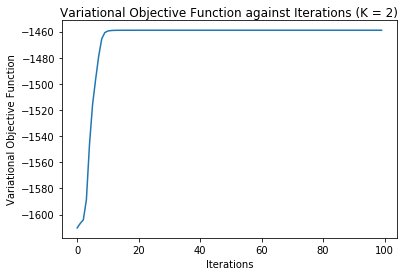
\includegraphics{VI_1}\\
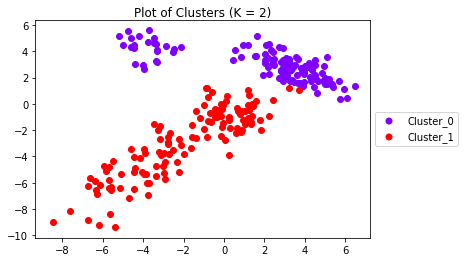
\includegraphics{VI_Plot_1}\\
\newpage
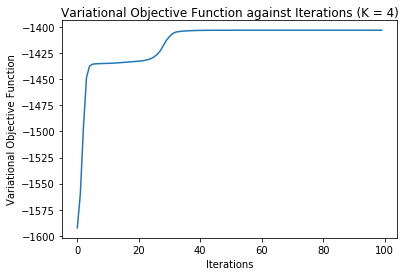
\includegraphics{VI_2}\\
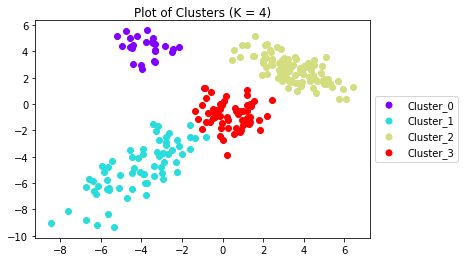
\includegraphics{VI_Plot_2}\\
\newpage
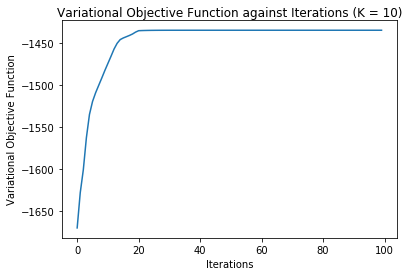
\includegraphics{VI_3}\\
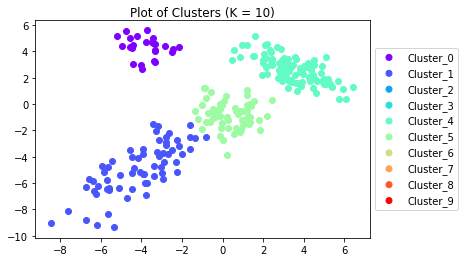
\includegraphics{VI_Plot_3}\\
\newpage
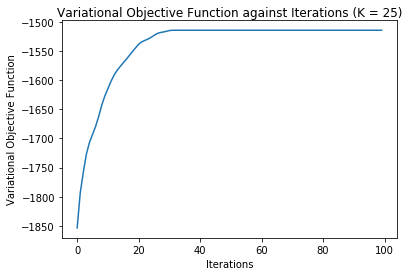
\includegraphics{VI_4}\\
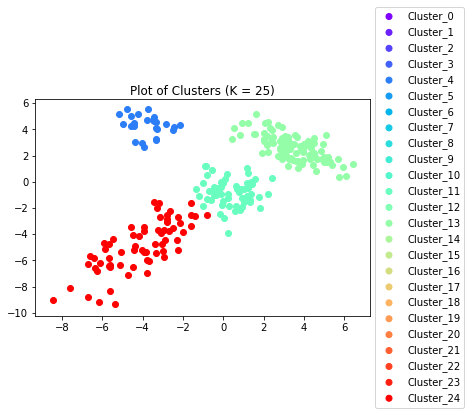
\includegraphics[scale=0.75]{VI_Plot_4}\\
\end{centering}
\newpage
\section*{Problem 3}
In our project, we will be the applying graphical models to problems of image segmentation and classification. Specifically, we will be working with the MNIST dataset [1] as it is fundamental benchmark in many image-related tasks. As the images in MNIST have undergone much preprocessing and are mostly noise-free, they do not reflect how real-world numbers are captured. Hence we will augment MNIST with random Gaussian noise to simulate such conditions. By construing image segmentation and classification of MNIST images as a graphical model, we would be able to obtain a posterior distributions over the images for each task which would enable us to deal with the injected noise. The goal of our project is two-fold: first we aim to separate the noisy images at the pixel as background and foreground; second, we classify the segmented image obtained from the previous step.

Our proposed model has 3 layers. The top 2 layers are responsible for segmentation and the bottom 2 for classification. Within the 2 layers responsible for segmentation, nodes in the top layer are observed and they correspond to pixels in the images which have values ranging from 0 to 255. The nodes in the bottom layer are hidden and there exists one hidden node for each observed node. Each of these nodes has a binary value that denotes whether the corresponding observed node belongs to the foreground or background and is connected to the observed node and its surrounding nodes. We impose a Dirichlet prior on the observed nodes and a multinomial likelihood on their values.

Classification is performed by the last two layers. The middle layer containing binary labels for the pixels can be thought of as a binarized version of the noisy image. We then have a single node in the bottom layer that is connected to every node in the middle layer. This node represents the class label for the digit.

Much recent work used binarized MNIST as a test set e.g. importance weighted autoencoders [2], NADE [3] and MADE [4] so we thought it would be a good idea apply to implement a simpler model and see how it compares against the state-of-the-art. \newline

\noindent
[1] LeCun, Y., Cortes, C. and Burges, C.J., 1998. The MNIST database of handwritten digits. \newline
[2] Burda, Y., Grosse, R. and Salakhutdinov, R., 2015. Importance weighted autoencoders. arXiv preprint arXiv:1509.00519. \newline
[3] Larochelle, H. and Murray, I., 2011. The Neural Autoregressive Distribution Estimator. In AISTATS (Vol. 1, p. 2). \newline
[4] Germain, M., Gregor, K., Murray, I. and Larochelle, H., 2015, February. Made: masked autoencoder for distribution estimation. In International Conference on Machine Learning (pp. 881-889).
\end{document}